% Options for packages loaded elsewhere
\PassOptionsToPackage{unicode}{hyperref}
\PassOptionsToPackage{hyphens}{url}
%
\documentclass[
]{article}
\usepackage{amsmath,amssymb}
\usepackage{iftex}
\ifPDFTeX
  \usepackage[T1]{fontenc}
  \usepackage[utf8]{inputenc}
  \usepackage{textcomp} % provide euro and other symbols
\else % if luatex or xetex
  \usepackage{unicode-math} % this also loads fontspec
  \defaultfontfeatures{Scale=MatchLowercase}
  \defaultfontfeatures[\rmfamily]{Ligatures=TeX,Scale=1}
\fi
\usepackage{lmodern}
\ifPDFTeX\else
  % xetex/luatex font selection
\fi
% Use upquote if available, for straight quotes in verbatim environments
\IfFileExists{upquote.sty}{\usepackage{upquote}}{}
\IfFileExists{microtype.sty}{% use microtype if available
  \usepackage[]{microtype}
  \UseMicrotypeSet[protrusion]{basicmath} % disable protrusion for tt fonts
}{}
\makeatletter
\@ifundefined{KOMAClassName}{% if non-KOMA class
  \IfFileExists{parskip.sty}{%
    \usepackage{parskip}
  }{% else
    \setlength{\parindent}{0pt}
    \setlength{\parskip}{6pt plus 2pt minus 1pt}}
}{% if KOMA class
  \KOMAoptions{parskip=half}}
\makeatother
\usepackage{xcolor}
\usepackage[margin=1in]{geometry}
\usepackage{color}
\usepackage{fancyvrb}
\newcommand{\VerbBar}{|}
\newcommand{\VERB}{\Verb[commandchars=\\\{\}]}
\DefineVerbatimEnvironment{Highlighting}{Verbatim}{commandchars=\\\{\}}
% Add ',fontsize=\small' for more characters per line
\usepackage{framed}
\definecolor{shadecolor}{RGB}{248,248,248}
\newenvironment{Shaded}{\begin{snugshade}}{\end{snugshade}}
\newcommand{\AlertTok}[1]{\textcolor[rgb]{0.94,0.16,0.16}{#1}}
\newcommand{\AnnotationTok}[1]{\textcolor[rgb]{0.56,0.35,0.01}{\textbf{\textit{#1}}}}
\newcommand{\AttributeTok}[1]{\textcolor[rgb]{0.13,0.29,0.53}{#1}}
\newcommand{\BaseNTok}[1]{\textcolor[rgb]{0.00,0.00,0.81}{#1}}
\newcommand{\BuiltInTok}[1]{#1}
\newcommand{\CharTok}[1]{\textcolor[rgb]{0.31,0.60,0.02}{#1}}
\newcommand{\CommentTok}[1]{\textcolor[rgb]{0.56,0.35,0.01}{\textit{#1}}}
\newcommand{\CommentVarTok}[1]{\textcolor[rgb]{0.56,0.35,0.01}{\textbf{\textit{#1}}}}
\newcommand{\ConstantTok}[1]{\textcolor[rgb]{0.56,0.35,0.01}{#1}}
\newcommand{\ControlFlowTok}[1]{\textcolor[rgb]{0.13,0.29,0.53}{\textbf{#1}}}
\newcommand{\DataTypeTok}[1]{\textcolor[rgb]{0.13,0.29,0.53}{#1}}
\newcommand{\DecValTok}[1]{\textcolor[rgb]{0.00,0.00,0.81}{#1}}
\newcommand{\DocumentationTok}[1]{\textcolor[rgb]{0.56,0.35,0.01}{\textbf{\textit{#1}}}}
\newcommand{\ErrorTok}[1]{\textcolor[rgb]{0.64,0.00,0.00}{\textbf{#1}}}
\newcommand{\ExtensionTok}[1]{#1}
\newcommand{\FloatTok}[1]{\textcolor[rgb]{0.00,0.00,0.81}{#1}}
\newcommand{\FunctionTok}[1]{\textcolor[rgb]{0.13,0.29,0.53}{\textbf{#1}}}
\newcommand{\ImportTok}[1]{#1}
\newcommand{\InformationTok}[1]{\textcolor[rgb]{0.56,0.35,0.01}{\textbf{\textit{#1}}}}
\newcommand{\KeywordTok}[1]{\textcolor[rgb]{0.13,0.29,0.53}{\textbf{#1}}}
\newcommand{\NormalTok}[1]{#1}
\newcommand{\OperatorTok}[1]{\textcolor[rgb]{0.81,0.36,0.00}{\textbf{#1}}}
\newcommand{\OtherTok}[1]{\textcolor[rgb]{0.56,0.35,0.01}{#1}}
\newcommand{\PreprocessorTok}[1]{\textcolor[rgb]{0.56,0.35,0.01}{\textit{#1}}}
\newcommand{\RegionMarkerTok}[1]{#1}
\newcommand{\SpecialCharTok}[1]{\textcolor[rgb]{0.81,0.36,0.00}{\textbf{#1}}}
\newcommand{\SpecialStringTok}[1]{\textcolor[rgb]{0.31,0.60,0.02}{#1}}
\newcommand{\StringTok}[1]{\textcolor[rgb]{0.31,0.60,0.02}{#1}}
\newcommand{\VariableTok}[1]{\textcolor[rgb]{0.00,0.00,0.00}{#1}}
\newcommand{\VerbatimStringTok}[1]{\textcolor[rgb]{0.31,0.60,0.02}{#1}}
\newcommand{\WarningTok}[1]{\textcolor[rgb]{0.56,0.35,0.01}{\textbf{\textit{#1}}}}
\usepackage{graphicx}
\makeatletter
\def\maxwidth{\ifdim\Gin@nat@width>\linewidth\linewidth\else\Gin@nat@width\fi}
\def\maxheight{\ifdim\Gin@nat@height>\textheight\textheight\else\Gin@nat@height\fi}
\makeatother
% Scale images if necessary, so that they will not overflow the page
% margins by default, and it is still possible to overwrite the defaults
% using explicit options in \includegraphics[width, height, ...]{}
\setkeys{Gin}{width=\maxwidth,height=\maxheight,keepaspectratio}
% Set default figure placement to htbp
\makeatletter
\def\fps@figure{htbp}
\makeatother
\setlength{\emergencystretch}{3em} % prevent overfull lines
\providecommand{\tightlist}{%
  \setlength{\itemsep}{0pt}\setlength{\parskip}{0pt}}
\setcounter{secnumdepth}{-\maxdimen} % remove section numbering
\usepackage{booktabs}
\usepackage{longtable}
\usepackage{array}
\usepackage{multirow}
\usepackage{wrapfig}
\usepackage{float}
\usepackage{colortbl}
\usepackage{pdflscape}
\usepackage{tabu}
\usepackage{threeparttable}
\usepackage{threeparttablex}
\usepackage[normalem]{ulem}
\usepackage{makecell}
\usepackage{xcolor}
\ifLuaTeX
  \usepackage{selnolig}  % disable illegal ligatures
\fi
\IfFileExists{bookmark.sty}{\usepackage{bookmark}}{\usepackage{hyperref}}
\IfFileExists{xurl.sty}{\usepackage{xurl}}{} % add URL line breaks if available
\urlstyle{same}
\hypersetup{
  pdftitle={Tarea 2 Estadística Actuarial II},
  pdfauthor={Maria Carolina Navarro Monge C05513; Tábata Picado Carmona C05961; Jose Pablo Trejos Conejo C07862},
  hidelinks,
  pdfcreator={LaTeX via pandoc}}

\title{Tarea 2 Estadística Actuarial II}
\author{Maria Carolina Navarro Monge C05513 \and Tábata Picado Carmona
C05961 \and Jose Pablo Trejos Conejo C07862}
\date{}

\begin{document}
\maketitle

\begin{Shaded}
\begin{Highlighting}[]
\CommentTok{\#Se cargan las librerías necesarias}
\FunctionTok{library}\NormalTok{(tidyverse)}
\FunctionTok{library}\NormalTok{(readxl)}
\FunctionTok{library}\NormalTok{(kableExtra)}
\end{Highlighting}
\end{Shaded}

\hypertarget{ejercicio-2}{%
\section{Ejercicio 2}\label{ejercicio-2}}

\textbf{Usando la metodología de Muestreo por Importancia, Si
X\textasciitilde N(0.5,0.5) estime:}

\hypertarget{a.-px-5}{%
\subsection{a. P(X\textless-5)}\label{a.-px-5}}

Primeramenre, mediante el metódo de integración por Montecarlo se
obtiene el siguiente resultado:

\begin{Shaded}
\begin{Highlighting}[]
\CommentTok{\#{-}{-}Estimación de función de distribución mediante integración por Montecarlo{-}{-}}

\FunctionTok{set.seed}\NormalTok{(}\DecValTok{2901}\NormalTok{)}
\NormalTok{n }\OtherTok{\textless{}{-}} \DecValTok{10}\SpecialCharTok{\^{}}\DecValTok{4} \CommentTok{\#tamaño de la muestra}

\NormalTok{X }\OtherTok{\textless{}{-}} \FunctionTok{rnorm}\NormalTok{(n, }\FloatTok{0.5}\NormalTok{, }\FunctionTok{sqrt}\NormalTok{(}\FloatTok{0.5}\NormalTok{))}

\NormalTok{f }\OtherTok{\textless{}{-}} \FunctionTok{dnorm}\NormalTok{(X, }\FloatTok{0.5}\NormalTok{, }\FunctionTok{sqrt}\NormalTok{(}\FloatTok{0.5}\NormalTok{))}

\NormalTok{valor\_estimado\_1 }\OtherTok{\textless{}{-}} \FunctionTok{mean}\NormalTok{(f)}

\NormalTok{valor\_real }\OtherTok{\textless{}{-}} \FunctionTok{pnorm}\NormalTok{(}\SpecialCharTok{{-}}\DecValTok{5}\NormalTok{, }\FloatTok{0.5}\NormalTok{, }\FunctionTok{sqrt}\NormalTok{(}\FloatTok{0.5}\NormalTok{))}

\NormalTok{comparacion }\OtherTok{\textless{}{-}} \FunctionTok{data.frame}\NormalTok{(}\StringTok{"Estimación"} \OtherTok{=}\NormalTok{ valor\_estimado\_1, }\StringTok{"Valor real"} \OtherTok{=}\NormalTok{ valor\_real)}

\CommentTok{\#kbl(comparacion)}
\FunctionTok{print}\NormalTok{(comparacion)}
\end{Highlighting}
\end{Shaded}

\begin{verbatim}
##   Estimación   Valor.real
## 1  0.3991698 3.678924e-15
\end{verbatim}

Como se puede observar, la estimación resultante converge lento al valor
real. Por lo tanto, mediante Muestreo por Importancia se puede acelelar
la convergencia empleando una densidad auxiliar. Para este caso, la
densidad auxiliar a utilizar es una exponencial truncada de la forma
\(\lambda e^{-\lambda(x-t)}\), con x\textgreater t.

La probabilidad a estimar es equivalente a P(X\textgreater6). Nos
basaremos en esta para aproximarla mediante el Muestro por Importancia
por medio de una exponencial truncada en 6 con \(\lambda = 1\). El
procedimiento se muestra en el siguiente algoritmo:

\begin{Shaded}
\begin{Highlighting}[]
\CommentTok{\#{-}{-}Estimación de función de distribución mediante Muestreo por Importancia{-}{-}}

\NormalTok{A }\OtherTok{\textless{}{-}} \FunctionTok{rexp}\NormalTok{(n)}\SpecialCharTok{+}\DecValTok{6} \CommentTok{\#datos aleatorios mayores a 6 con distribución exponencial}

\NormalTok{w }\OtherTok{\textless{}{-}} \FunctionTok{dnorm}\NormalTok{(A, }\FloatTok{0.5}\NormalTok{, }\FunctionTok{sqrt}\NormalTok{(}\FloatTok{0.5}\NormalTok{)) }\SpecialCharTok{/} \FunctionTok{dexp}\NormalTok{(A}\DecValTok{{-}6}\NormalTok{)}

\NormalTok{valor\_estimado }\OtherTok{\textless{}{-}} \FunctionTok{mean}\NormalTok{(w)}

\NormalTok{resumen }\OtherTok{\textless{}{-}} \FunctionTok{data.frame}\NormalTok{(}\StringTok{"Estimación"} \OtherTok{=}\NormalTok{ valor\_estimado, }\StringTok{"Valor real"} \OtherTok{=}\NormalTok{ valor\_real)}

\CommentTok{\#kbl(resumen)}
\FunctionTok{print}\NormalTok{(resumen)}
\end{Highlighting}
\end{Shaded}

\begin{verbatim}
##     Estimación   Valor.real
## 1 3.669418e-15 3.678924e-15
\end{verbatim}

De tal manera, se obtiene una mejor aproximación de la probabilidad
P(X\textless-5), pues, es muy similar al valor real.

\hypertarget{b.-estime-el-error-absoluto-de-la-estimaciuxf3n-del-punto-a.}{%
\subsection{b. Estime el error absoluto de la estimación del punto
a.}\label{b.-estime-el-error-absoluto-de-la-estimaciuxf3n-del-punto-a.}}

El error absoluto de la estimación es:

\begin{Shaded}
\begin{Highlighting}[]
\NormalTok{error\_absoluto }\OtherTok{\textless{}{-}} \FunctionTok{abs}\NormalTok{(valor\_estimado}\SpecialCharTok{{-}}\NormalTok{valor\_real)}
\end{Highlighting}
\end{Shaded}

\#Ejercicio 5

\textbf{Una aseguradora tiene un producto llamado Doble Seguro de Vida
(DSV) el cual paga 2 veces la suma asegurada si la persona fallece antes
de los 60 años, paga 1 suma asegurada cuando la persona cumple los 60
años (si no ha fallecido) y paga 1 suma asegurada si fallece después de
los 60 años. Considerando:}

\textbf{a. Las tablas de vida dinámicas de la SUPEN
(\url{https://webapps.supen.fi.cr/tablasVida/Recursos/documentos/tavid2000-2150.xls})}

\textbf{b. Un cliente de 30 años, hombre con una suma asegurable de 1
000 000 colones.}

\textbf{Construya con la ayuda de un MCMC la distribución de los pagos
por año de que se espera de este seguro. Use al menos 10 000
iteraciones. Y muestre Histograma.}

Primeramente, se carga la tabla de vida dinámica de la SUPEN y se filtra
para obtener los datos correspondientes para un hombre que en el
presente año (2024) tiene 30 años

\begin{Shaded}
\begin{Highlighting}[]
\CommentTok{\#Se carga la base de datos}
\NormalTok{tabla\_vida }\OtherTok{\textless{}{-}} \FunctionTok{read\_excel}\NormalTok{(}\StringTok{"tavid2000{-}2150.xls"}\NormalTok{,}
                         \AttributeTok{col\_types =} \StringTok{"numeric"}\NormalTok{)}

\CommentTok{\#Se filtra la base de datos para obtener los datos de un hombre nacido en 1994 }
\CommentTok{\#con edades mayor o igual a 30}

\NormalTok{datos }\OtherTok{\textless{}{-}} \FunctionTok{subset}\NormalTok{(tabla\_vida, sex }\SpecialCharTok{==} \DecValTok{1} \SpecialCharTok{\&}\NormalTok{ ynac }\SpecialCharTok{==} \DecValTok{1994} \SpecialCharTok{\&}\NormalTok{ edad }\SpecialCharTok{\textgreater{}=}\DecValTok{30}\NormalTok{, }\AttributeTok{select =} \FunctionTok{c}\NormalTok{(edad,qx, year))}
\end{Highlighting}
\end{Shaded}

Además, se calculan las probabilidades de sobrevivencia necesarias para
procesos posteriores

\begin{Shaded}
\begin{Highlighting}[]
\CommentTok{\#Se obtienen las probabilidades de sobrevivencia}

\NormalTok{px }\OtherTok{\textless{}{-}} \DecValTok{1}\SpecialCharTok{{-}}\NormalTok{ datos}\SpecialCharTok{$}\NormalTok{qx}

\CommentTok{\#Se añaden las probabilidades de sobrevivencia a la base datos}
\NormalTok{datos}\SpecialCharTok{$}\NormalTok{px }\OtherTok{\textless{}{-}}\NormalTok{ px}
\end{Highlighting}
\end{Shaded}

La construcción de la distribución de los pagos por año mediante MCMC se
muestran en el siguiente código:

\begin{Shaded}
\begin{Highlighting}[]
\NormalTok{suma\_asegurada\_1 }\OtherTok{\textless{}{-}} \DecValTok{10}\SpecialCharTok{\^{}}\DecValTok{6}
\NormalTok{suma\_asegurada\_2 }\OtherTok{\textless{}{-}} \DecValTok{2}\SpecialCharTok{*}\DecValTok{10}\SpecialCharTok{\^{}}\DecValTok{6}

\CommentTok{\#{-}{-}{-}{-}{-}{-}{-}{-}{-}{-}{-}{-}{-}{-}{-}{-}{-}{-}{-}{-}MCMC{-}{-}{-}{-}{-}{-}{-}{-}{-}{-}{-}{-}{-}{-}{-}{-}{-}{-}{-}{-}{-}{-}{-}{-}{-}{-}{-}{-}{-}{-}{-}{-}{-}|   }

\CommentTok{\#Se simulan diversas trayectorias de vida de la persona}
\FunctionTok{set.seed}\NormalTok{(}\DecValTok{2901}\NormalTok{)}
\NormalTok{iteraciones}\OtherTok{=}\DecValTok{10}\SpecialCharTok{\^{}}\DecValTok{4}
\NormalTok{n}\OtherTok{=}\FunctionTok{length}\NormalTok{(px)}
\NormalTok{pago }\OtherTok{\textless{}{-}} \FunctionTok{rep}\NormalTok{(}\DecValTok{0}\NormalTok{, }\DecValTok{86}\NormalTok{)}

\ControlFlowTok{for}\NormalTok{ (i }\ControlFlowTok{in} \DecValTok{1}\SpecialCharTok{:}\NormalTok{iteraciones) \{}
\NormalTok{  U }\OtherTok{\textless{}{-}} \FunctionTok{runif}\NormalTok{(n)  }\CommentTok{\# Se toman como probabilidades de muerte}
\NormalTok{  t }\OtherTok{\textless{}{-}} \DecValTok{1}
\NormalTok{  cont }\OtherTok{\textless{}{-}} \DecValTok{1}
  
  \CommentTok{\#Determinación del año de fallecimiento}
  \ControlFlowTok{while}\NormalTok{ (t }\SpecialCharTok{==} \DecValTok{1}\NormalTok{) \{}
    \ControlFlowTok{if}\NormalTok{ (U[cont] }\SpecialCharTok{\textless{}}\NormalTok{ px[cont]) \{}
\NormalTok{      cont }\OtherTok{\textless{}{-}}\NormalTok{ cont }\SpecialCharTok{+} \DecValTok{1}
\NormalTok{    \} }\ControlFlowTok{else}\NormalTok{ \{}
\NormalTok{      t }\OtherTok{\textless{}{-}} \DecValTok{0}
\NormalTok{    \}}
\NormalTok{  \}}
\NormalTok{  año\_fallecimiento }\OtherTok{\textless{}{-}}\NormalTok{ cont }\SpecialCharTok{{-}} \DecValTok{1}
  
  \CommentTok{\#Asignar los pagos correspondientes al año de fallecimiento}
  \ControlFlowTok{if}\NormalTok{ (año\_fallecimiento }\SpecialCharTok{\textless{}} \DecValTok{30}\NormalTok{) \{}
\NormalTok{    pago[año\_fallecimiento }\SpecialCharTok{+} \DecValTok{1}\NormalTok{] }\OtherTok{\textless{}{-}}\NormalTok{ pago[año\_fallecimiento }\SpecialCharTok{+} \DecValTok{1}\NormalTok{] }\SpecialCharTok{+}\NormalTok{ suma\_asegurada\_2 }
\NormalTok{  \} }\ControlFlowTok{else} \ControlFlowTok{if}\NormalTok{ (año\_fallecimiento }\SpecialCharTok{==}\DecValTok{30}\NormalTok{) \{}
\NormalTok{    pago[}\DecValTok{31}\NormalTok{] }\OtherTok{\textless{}{-}}\NormalTok{ pago[}\DecValTok{31}\NormalTok{]}\SpecialCharTok{+}\NormalTok{ suma\_asegurada\_1}
\NormalTok{  \}}\ControlFlowTok{else}\NormalTok{ \{}
\NormalTok{    pago[}\DecValTok{31}\NormalTok{] }\OtherTok{\textless{}{-}}\NormalTok{ pago[}\DecValTok{31}\NormalTok{] }\SpecialCharTok{+}\NormalTok{ suma\_asegurada\_1 }
\NormalTok{    pago[año\_fallecimiento }\SpecialCharTok{+} \DecValTok{1}\NormalTok{] }\OtherTok{\textless{}{-}}\NormalTok{ pago[año\_fallecimiento }\SpecialCharTok{+} \DecValTok{1}\NormalTok{] }\SpecialCharTok{+}\NormalTok{ suma\_asegurada\_1}
\NormalTok{  \}}
\NormalTok{\}}

\NormalTok{resultado }\OtherTok{\textless{}{-}} \FunctionTok{data.frame}\NormalTok{(}\StringTok{"Años pago"}\OtherTok{=}\NormalTok{ datos}\SpecialCharTok{$}\NormalTok{year, }\StringTok{"Pago"} \OtherTok{=}\NormalTok{ pago)}
\end{Highlighting}
\end{Shaded}

El histograma de los pagos esperados por año es el siguiente:

\begin{Shaded}
\begin{Highlighting}[]
\FunctionTok{ggplot}\NormalTok{(}\AttributeTok{data =}\NormalTok{ resultado, }\FunctionTok{aes}\NormalTok{(}\AttributeTok{x =}\NormalTok{ Años.pago, }\AttributeTok{y =}\NormalTok{ Pago)) }\SpecialCharTok{+}  
  \FunctionTok{geom\_bar}\NormalTok{(}\AttributeTok{stat =} \StringTok{"identity"}\NormalTok{, }\AttributeTok{fill =} \StringTok{"blue"}\NormalTok{) }\SpecialCharTok{+}  
  \FunctionTok{labs}\NormalTok{(}\AttributeTok{title =} \StringTok{"Histograma de Pagos Esperados por año"}\NormalTok{, }\AttributeTok{x =} \StringTok{"Años"}\NormalTok{, }\AttributeTok{y =} \StringTok{"Frecuencia"}\NormalTok{)}\SpecialCharTok{+}
  \FunctionTok{theme\_minimal}\NormalTok{()}
\end{Highlighting}
\end{Shaded}

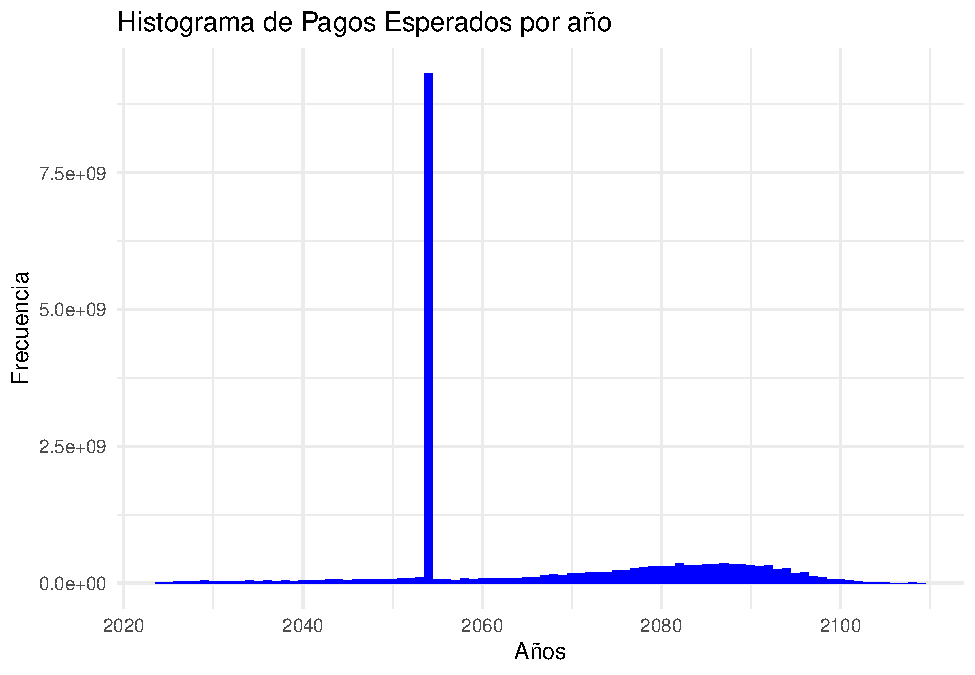
\includegraphics{Rmarkdown_files/figure-latex/unnamed-chunk-8-1.pdf}

Es evidente que la mayor cantidad de pagos se sitúan a los 60 años y
posteriomente después de los 60, lo que indica que es más probable que
el cliente fallezca después de los 60 años.

Se puede verificar el resultado obtenido por MCMC si lo comparamos con
un histograma obtenido mediante un método determinista como el que se
muestra a continuación:

\begin{Shaded}
\begin{Highlighting}[]
\CommentTok{\#{-}{-}{-}{-}{-} Método determinista{-}{-}{-}{-}{-}{-}{-}{-}{-}{-}{-}{-}{-}{-}{-}{-}{-}{-}{-}{-}{-}{-}{-}{-}{-}{-}{-}{-}{-}{-}{-}{-}{-}{-}{-}{-}{-}{-}{-}{-}{-}{-}{-}{-}{-}{-}{-}{-}{-}{-}{-}{-}{-}|}

\NormalTok{qx}\OtherTok{\textless{}{-}}\NormalTok{ datos}\SpecialCharTok{$}\NormalTok{qx}

\CommentTok{\#Se crea una función que obtiene n\_p\_30 (probabilidad de sobrevivencia acumulada)}
\NormalTok{n\_p\_30 }\OtherTok{\textless{}{-}} \FunctionTok{c}\NormalTok{(}\DecValTok{0}\NormalTok{)}

\NormalTok{n\_p\_30\_function }\OtherTok{\textless{}{-}} \ControlFlowTok{function}\NormalTok{(px) \{}

  \ControlFlowTok{for}\NormalTok{ (i }\ControlFlowTok{in} \DecValTok{1}\SpecialCharTok{:}\FunctionTok{length}\NormalTok{(px)) \{}
\NormalTok{    resultado }\OtherTok{\textless{}{-}}\DecValTok{1}
    \ControlFlowTok{for}\NormalTok{(j }\ControlFlowTok{in} \DecValTok{1}\SpecialCharTok{:}\NormalTok{ i)\{}
\NormalTok{      resultado }\OtherTok{\textless{}{-}}\NormalTok{ resultado}\SpecialCharTok{*}\NormalTok{px[j]}
\NormalTok{    \}}
    
\NormalTok{    n\_p\_30[i] }\OtherTok{\textless{}{-}}\NormalTok{ resultado}
\NormalTok{  \}}
  
  \FunctionTok{return}\NormalTok{(n\_p\_30)}
\NormalTok{\}}

\NormalTok{n\_p\_30 }\OtherTok{\textless{}{-}} \FunctionTok{n\_p\_30\_function}\NormalTok{(px)}

\NormalTok{datos}\SpecialCharTok{$}\NormalTok{n\_p\_30 }\OtherTok{\textless{}{-}}\NormalTok{ n\_p\_30 }


\CommentTok{\#se calculan los pagos esperados para cada año}
\NormalTok{pago\_esperado }\OtherTok{\textless{}{-}} \FunctionTok{c}\NormalTok{(}\DecValTok{0}\NormalTok{)}
\NormalTok{pago\_esperado[}\DecValTok{1}\NormalTok{] }\OtherTok{\textless{}{-}}\NormalTok{ suma\_asegurada\_2}\SpecialCharTok{*}\NormalTok{qx[}\DecValTok{1}\NormalTok{]}

\CommentTok{\#caso fallecimiento antes de los 60 años}
\ControlFlowTok{for}\NormalTok{ (i }\ControlFlowTok{in} \DecValTok{2}\SpecialCharTok{:} \DecValTok{29}\NormalTok{ ) \{}
\NormalTok{    pago\_esperado[i] }\OtherTok{\textless{}{-}}\NormalTok{ suma\_asegurada\_2}\SpecialCharTok{*}\NormalTok{n\_p\_30[i}\DecValTok{{-}1}\NormalTok{]}\SpecialCharTok{*}\NormalTok{qx[i]}
\NormalTok{\}}

\CommentTok{\#caso sobrevive a los 60 años}

\NormalTok{pago\_esperado[}\DecValTok{30}\NormalTok{] }\OtherTok{\textless{}{-}}\NormalTok{suma\_asegurada\_1}\SpecialCharTok{*}\NormalTok{n\_p\_30[}\DecValTok{30}\NormalTok{]}

\CommentTok{\#caso fallecimiento después de los 60 años}

\ControlFlowTok{for}\NormalTok{ (i }\ControlFlowTok{in} \DecValTok{1}\SpecialCharTok{:}\NormalTok{ (}\FunctionTok{length}\NormalTok{(px)}\SpecialCharTok{{-}}\DecValTok{30}\NormalTok{)) \{}
\NormalTok{  pago\_esperado[}\DecValTok{30}\SpecialCharTok{+}\NormalTok{i] }\OtherTok{\textless{}{-}}\NormalTok{ suma\_asegurada\_1}\SpecialCharTok{*}\NormalTok{n\_p\_30[}\DecValTok{30}\SpecialCharTok{+}\NormalTok{i}\DecValTok{{-}1}\NormalTok{]}\SpecialCharTok{*}\NormalTok{qx[}\DecValTok{30}\SpecialCharTok{+}\NormalTok{i]}
\NormalTok{\}}

\NormalTok{resultado\_determinista }\OtherTok{\textless{}{-}} \FunctionTok{data.frame}\NormalTok{(}\StringTok{"Años pago"}\OtherTok{=}\NormalTok{ datos}\SpecialCharTok{$}\NormalTok{year, }\StringTok{"Pago"} \OtherTok{=}\NormalTok{ pago\_esperado)}
 
\FunctionTok{ggplot}\NormalTok{(}\AttributeTok{data =}\NormalTok{ resultado\_determinista, }\FunctionTok{aes}\NormalTok{(}\AttributeTok{x =}\NormalTok{ Años.pago, }\AttributeTok{y =}\NormalTok{ Pago)) }\SpecialCharTok{+}  
  \FunctionTok{geom\_bar}\NormalTok{(}\AttributeTok{stat =} \StringTok{"identity"}\NormalTok{, }\AttributeTok{fill =} \StringTok{"blue"}\NormalTok{) }\SpecialCharTok{+}  
  \FunctionTok{labs}\NormalTok{(}\AttributeTok{title =} \StringTok{"Histograma de Pagos Esperados por año"}\NormalTok{, }\AttributeTok{x =} \StringTok{"Años"}\NormalTok{, }\AttributeTok{y =} \StringTok{"Frecuencia"}\NormalTok{)}\SpecialCharTok{+}
  \FunctionTok{theme\_minimal}\NormalTok{()}
\end{Highlighting}
\end{Shaded}

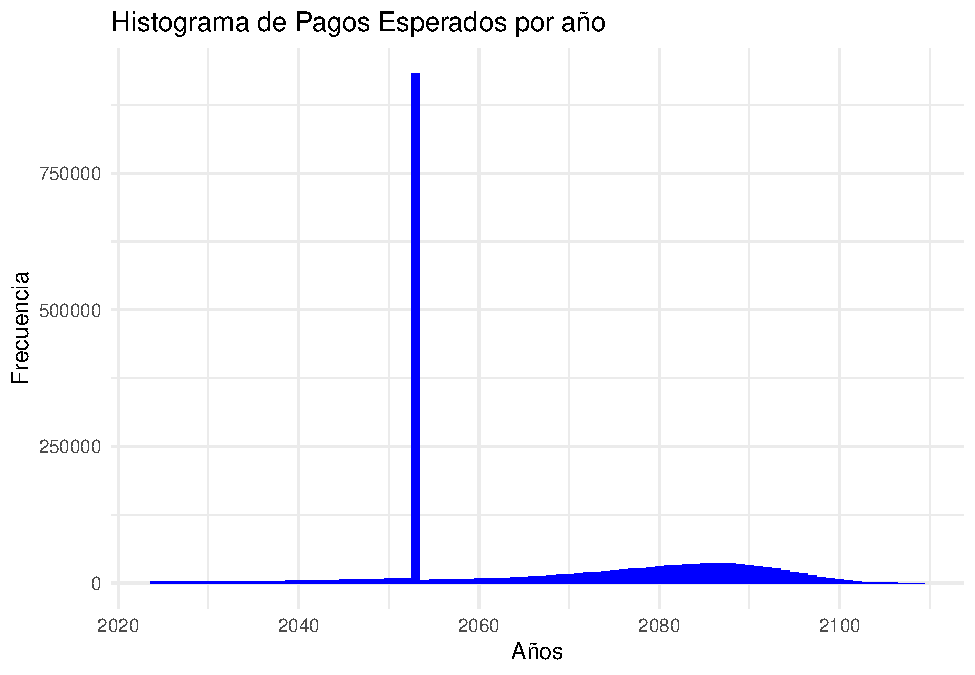
\includegraphics{Rmarkdown_files/figure-latex/unnamed-chunk-9-1.pdf}

Como se puede observar, los pagos esperados mediante el método
determinista y el MCMC muestran distribuciones muy similares. Por tanto,
se verifica que el resultado que se obtuvo por el método MCMC es
aceptable.

\end{document}
